%%%%%%%%%%%%%%%%%%%%%%%%%%%%%%%%%%%%%%%%%%%%%%%%%%%%%%%%%%%%%%%%%%%%%
%% This is a (brief) model paper using the achemso class
%% The document class accepts keyval options, which should include
%% the target journal and optionally the manuscript type. 
%%%%%%%%%%%%%%%%%%%%%%%%%%%%%%%%%%%%%%%%%%%%%%%%%%%%%%%%%%%%%%%%%%%%%
\documentclass[journal=jacsat,manuscript=article]{achemso}

%%%%%%%%%%%%%%%%%%%%%%%%%%%%%%%%%%%%%%%%%%%%%%%%%%%%%%%%%%%%%%%%%%%%%
%% Place any additional packages needed here.  Only include packages
%%, which are essential, to avoid problems later. Do NOT use any
%% packages which require e-TeX (for example etoolbox): the e-TeX
%% extensions are not currently available on the ACS conversion
%% servers.
%%%%%%%%%%%%%%%%%%%%%%%%%%%%%%%%%%%%%%%%%%%%%%%%%%%%%%%%%%%%%%%%%%%%%
% \usepackage[version=3]{mhchem} % Formula subscripts using \ce{}
\usepackage{hyperref}
\usepackage{graphicx}
\usepackage{array}

\graphicspath{ {./resources/} }
\newcolumntype{P}[1]{>{\centering\arraybackslash}p{#1}}


%%%%%%%%%%%%%%%%%%%%%%%%%%%%%%%%%%%%%%%%%%%%%%%%%%%%%%%%%%%%%%%%%%%%%
%% If issues arise when submitting your manuscript, you may want to
%% un-comment the next line.  This provides information on the
%% version of every file you have used.
%%%%%%%%%%%%%%%%%%%%%%%%%%%%%%%%%%%%%%%%%%%%%%%%%%%%%%%%%%%%%%%%%%%%%
%%\listfiles

%%%%%%%%%%%%%%%%%%%%%%%%%%%%%%%%%%%%%%%%%%%%%%%%%%%%%%%%%%%%%%%%%%%%%
%% Place any additional macros here.  Please use \newcommand* where
%% possible, and avoid layout-changing macros (which are not used
%% when typesetting).
%%%%%%%%%%%%%%%%%%%%%%%%%%%%%%%%%%%%%%%%%%%%%%%%%%%%%%%%%%%%%%%%%%%%%
\newcommand*\mycommand[1]{\texttt{\emph{#1}}}
\renewcommand{\thefootnote}{\fnsymbol{footnote}}

\author{Vineeth R. Chelur}
\author{U. Deva Priyakumar}
\email{deva@iiit.ac.in}
% \phone{+91 9490441430}
% \author{Yashaswi Pathak}
\affiliation[IIIT-H]
{Center for Computational Natural Sciences \& Bioinformatics, IIIT-H, Hyderabad}

%%%%%%%%%%%%%%%%%%%%%%%%%%%%%%%%%%%%%%%%%%%%%%%%%%%%%%%%%%%%%%%%%%%%%
%% The document title should be given as usual. Some journals require
%% a running title from the author: this should be supplied as an
%% optional argument to \title.
%%%%%%%%%%%%%%%%%%%%%%%%%%%%%%%%%%%%%%%%%%%%%%%%%%%%%%%%%%%%%%%%%%%%%
\title[Predicting the binding-site of a protein for druggable ligands from sequence-based features using Deep Learning]
  {Predicting the binding-site of a protein for druggable ligands from sequence-based features using Deep Learning
%   \footnote{A footnote for the title}
  }

%%%%%%%%%%%%%%%%%%%%%%%%%%%%%%%%%%%%%%%%%%%%%%%%%%%%%%%%%%%%%%%%%%%%%
%% Some journals require a list of abbreviations or keywords to be
%% supplied. These should be set up here, and will be printed after
%% the title and author information, if needed.
%%%%%%%%%%%%%%%%%%%%%%%%%%%%%%%%%%%%%%%%%%%%%%%%%%%%%%%%%%%%%%%%%%%%%
% \abbreviations{IR,NMR,UV}
% \keywords{American Chemical Society, \LaTeX}

%%%%%%%%%%%%%%%%%%%%%%%%%%%%%%%%%%%%%%%%%%%%%%%%%%%%%%%%%%%%%%%%%%%%%
%% The manuscript does not need to include \maketitle, which is
%% executed automatically.
%%%%%%%%%%%%%%%%%%%%%%%%%%%%%%%%%%%%%%%%%%%%%%%%%%%%%%%%%%%%%%%%%%%%%
\begin{document}

%%%%%%%%%%%%%%%%%%%%%%%%%%%%%%%%%%%%%%%%%%%%%%%%%%%%%%%%%%%%%%%%%%%%%
%% The "tocentry" environment can be used to create an entry for the
%% graphical table of contents. It is given here as some journals
%% require that it is printed as part of the abstract page. It will
%% be automatically moved as appropriate.
%%%%%%%%%%%%%%%%%%%%%%%%%%%%%%%%%%%%%%%%%%%%%%%%%%%%%%%%%%%%%%%%%%%%%
% \begin{tocentry}

% Some journals require a graphical entry for the Table of Contents.
% This should be laid out ``print ready'' so that the sizing of the
% text is correct.

% Inside the \texttt{tocentry} environment, the font used is Helvetica
% 8\,pt, as required by \emph{Journal of the American Chemical
% Society}.

% The surrounding frame is 9\,cm by 3.5\,cm, which is the maximum
% permitted for  \emph{Journal of the American Chemical Society}
% graphical table of content entries. The box will not resize if the
% content is too big: instead it will overflow the edge of the box.

% This box and the associated title will always be printed on a
% separate page at the end of the document.

% \end{tocentry}

%%%%%%%%%%%%%%%%%%%%%%%%%%%%%%%%%%%%%%%%%%%%%%%%%%%%%%%%%%%%%%%%%%%%%
%% The abstract environment will automatically gobble the contents
%% if an abstract is not used by the target journal.
%%%%%%%%%%%%%%%%%%%%%%%%%%%%%%%%%%%%%%%%%%%%%%%%%%%%%%%%%%%%%%%%%%%%%
\begin{abstract}
    \noindent\textbf{Motivation}: Protein-drug interactions play important roles in many biological processes. The prediction of the active binding site of a protein helps discover such interactions. The tertiary structure of a protein determines the binding sites available to the drug molecule. But the methods for structure determination are labour-intensive and time-consuming. Hence it becomes important to make predictions using the sequence alone. Deep Learning has been used in a variety of biochemical tasks and has been hugely successful. In this paper, a residual neural network is implemented to predict a protein's most active binding site using features extracted from just the sequence.

    \noindent\textbf{Results}: The model achieves an MCC of 0.52 and an accuracy of 92.2\% on the validation sets averaging across 10-folds. On the test set, the prediction of 10 models aggregated give an MCC of 0.55 and an accuracy of 94.1\%.

    \noindent\textbf{Implementation}: \href{https://github.com/crvineeth97/protein-binding-site-prediction}{https://github.com/crvineeth97/protein-binding-site-prediction}
\end{abstract}

%%%%%%%%%%%%%%%%%%%%%%%%%%%%%%%%%%%%%%%%%%%%%%%%%%%%%%%%%%%%%%%%%%%%%
%% Start the main part of the manuscript here.
%%%%%%%%%%%%%%%%%%%%%%%%%%%%%%%%%%%%%%%%%%%%%%%%%%%%%%%%%%%%%%%%%%%%%
\section{Introduction}
\quad The rapid speed of sequencing attained with modern DNA sequencing technology has been instrumental in the sequencing of complete DNA sequences, which leads to faster indirect sequencing of proteins. Although there have been improvements in the determination of the three-dimensional protein structure by techniques such as X-ray crystallography and NMR Spectroscopy, the gap between the number of known sequences (333,201,385 as of July 2020) and the number of known structures (154,706 as of July 2020) is increasing rapidly. Proteins perform a vast array of functions within organisms, and the tertiary structure of a protein can provide important clues about these functions.

Deep Learning is a subfield of machine learning based on artificial neural networks with feature learning. When a deep learning model is fed large amounts of data, it can automatically discover the representations needed for feature detection or classification. Deep learning has been hugely successful in all fields of Natural Sciences, including, but not limited to, binding affinity predictions, protein contact map predictions, and protein-structure predictions. For example, Google's DeepMind team designed a deep learning model, called AlphaFold \cite{senior2020improved}, which represents a considerable advance in protein-structure prediction from a sequence.

In the process of drug design, new medications are found based on the knowledge of a biological target such as a protein. The identification of the potential active binding site of a protein is an essential step in drug design. Predicting the binding site of a protein, based on sequence alone, becomes critical when the three-dimensional structure of the protein is not available.

In this paper, a deep residual neural network is trained to make the binary prediction of whether an amino acid residue of the sequence belongs to the primary binding site or not.

\section{Dataset}
\quad For the training and validation of the model, the sc-PDB\cite{desaphy2015sc} dataset (v 2017) is used. The database consists of druggable binding sites of the Protein Data Bank along with prepared protein structures. Thus each sample in the dataset contains the three-dimensional structure of one ligand, one protein, and one site, all stored in mol2 format.

Typically, the complete structure of a protein is unavailable due to missing residues, and hence the full sequence of the protein is obtained from RCSB \cite{burley2019rcsb} website\footnote{Some PDBs in the dataset were obsoleted, and hence the sequences were manually tracked on RCSB, and the corresponding sequences were used. List of obsoleted PDBs is provided in Supporting Information}. A one-to-one mapping of the amino acids in the sequence to the one in the protein mol2 file is required, to know which amino acid belongs to a binding site. This mapping is done by first extracting the protein sequence from the 3D structure. Next, the Needleman-Wunsch dynamic programming algorithm is used to align the sequence extracted from the structure file to the downloaded RCSB sequence. This algorithm is implemented using a modified version of Zhanglab's NW-Align program\cite{NWAlign}. The protein structure file is then reindexed, based on this alignment, to match the indexing of the RCSB sequence. This way, the specific binding residues can be labelled in the RCSB sequence.


The training set consists of 17,594 PDB structures with 28,959 sequences (9519 unique sequences), originating from 1240 organisms, the most abundant being humans(28.26\%). The dataset was diverse and contained proteins from 1996 different PFAM families and 856 PFAM clans.

\begin{table}
    \centering
    \begin{tabular}{| P{2.75cm} | P{2.75cm} | P{2.75cm} | P{2.75cm} | P{2.75cm} |}
        \hline
              & $N_{prot}$ & $N_{br}$ & $N_{nbr}$ & $P_{br}(\%)$ \\
        \hline
        Train & 15,860     & 589,329  & 8,725,043 & 6.33         \\
        % Valid & 1586       &          &           &              \\
        Test  & 2,464      & 86,230   & 1,345,646 & 6.02         \\
        \hline
    \end{tabular}
    \caption{\label{tab:dataset_summary} Summary of the datasets}
    \vspace{5 mm}
    \noindent $N_{prot}$ - Number of proteins \hfill $N_{br}$ - Total number of binding residues

    \vspace{3 mm}

    \noindent $N_{nbr}$ - Total number of non-binding residues \hfill $P_{br}(\%)$ - Percentage of binding residues
\end{table}

This data is split into 10-folds (each containing 1586 structures), based on Uniprot ID, exactly like how \citeauthor{stepniewska2020improving} did in their paper \cite{stepniewska2020improving}. This split ensures that there is no data leakage between the validation and training set by putting all structures of a single protein in the same fold.

The test set is constructed using all PDBs from 2018 onwards, till 28th February 2020. All PDBs available during this period and having at least one ligand are considered. These are then run through the pdbconv tool from the IChem Toolkit \cite{da2018ichem} to generate a dataset with the same filters and site selection as the sc-PDB training set.

The test set consists of 2,274 PDB structures with 3,434 sequences (1889 unique sequences), originating from 548 organisms, the most abundant being human(23.76\%). The test set contained proteins from 882 PFAM families and 452 PFAM clans.


\section{Methods}
\subsection{MSA Generation}
\quad Collections of multiple homologous sequences (called Multiple Sequence Alignments or MSAs) can provide critical information for the modelling of the structure and function of unknown proteins. DeepMSA \cite{zhang2020deepmsa} is an open-source method for sensitive MSA construction, which has homologous sequences and alignments created from multiple sources of databases through complementary hidden Markov model algorithms.

The search is done in 2 stages. In stage 1, the query sequence is searched against the UniClust30 \cite{mirdita2017uniclust} database using HHBlits from HH-suite\cite{remmert2012hhblits} (v2.0.16). If the number of effective sequences is $<$ 128, Stage 2 is performed where the query sequence is searched against the Uniref50 \cite{suzek2015uniref} database using JackHMMER from HMMER \cite{johnson2010hidden} (v3.1b2). Full-length sequences are extracted from the JackHMMER raw hits and converted into a custom HHBlits format database. HHBlits is applied to jump-start the search from Stage 1 sequence MSA against this custom database.


\subsection{Features}
\quad There are 9519 unique protein sequences in the sc-PDB dataset and 1889 unique protein sequences in the test set. The MSAs are generated for these sequences using the method described above and stored in PSICOV \cite{jones2012psicov} .aln format.

One-hot encoding and Postional embeddings are extracted from the sequence alone. Position Specific Scoring Matrix, Information Content, Secondary Structure and Solvent Accessibility are extracted from the generated MSAs.

\subsubsection{One-hot encoding and Positional embeddings}
\quad There are 20 standard amino acids and the non-standard amino acids are all labelled as an additional dummy residue, X. This leads to 21 amino acids in our vocabulary. The 20 standard amino acids are used in alphabetical order, numbered from 1 to 20, and the dummy residue X is given the position 0. The one-hot encoding (OHE) of an amino acid will be a vector of zeroes of length 21, where the position of the amino acid in the vocabulary is marked with a one. This is used to help the model differentiate between the different types of amino acids

Positional  (PE) carry information about the absolute position of the amino acids in the sequence. A simple method of embedding is used where the position of the $i^{th}$ amino acid is represented by ${PE}_{i} = \frac{i}{L}$ where L is the length of the protein sequence.

\subsubsection{Position Specific Scoring Matrix and Information Content}
\quad Position Specific Scoring Matrix (PSSM) is a commonly used representation of patterns in biological sequences. PSSMs are derived from MSAs using Easel \cite{potter2018hmmer} and Heinikoff position-based weights so that similar sequences collectively contributed less to PSSM probabilities than diverse sequences.

The information content (IC) of a PSSM gives an idea about how different the PSSM is from a uniform distribution. IC is also derived using Easel.

\subsubsection{Secondary Structure and Solvent Accessibility}
\quad The secondary structure is defined by the pattern of hydrogen bonds formed between the amino hydrogen and carboxyl oxygen atoms in the peptide backbone. It gives an idea of the three-dimensional structure of the protein. The secondary structural elements are alpha helices, beta sheets and turns. PSIPRED (v4.0) \cite{jones1999protein} is used to predict the probability of each state of the 3-state secondary structure (SS3) for every amino acid in the sequence.

The solvent-accessible surface area is the surface area of a biomolecule that is accessible to a solvent. SOLVPRED from MetaPSICOV 2.0\cite{jones2015metapsicov} is used to predict the relative solvent accessibility (RSA) of every amino acid in the sequence. RSA can be calculated as \\ ${RSA} = {ASA} / {MaxASA}$, where ASA is the solvent-accessible surface area, and MaxASA is the maximum possible solvent accessible surface area for the amino acid residue.

% \subsubsection{SPOT-1D Features}
% \quad As a means to provide better features, SPOT-1D \cite{hanson2019improving} was used to generate the following features: solvent accessibility, half-sphere exposure, contact number, 3-state secondary structure, 8-state secondary structure, and phi, psi, theta and tau torsion angles.

% The first step in the prediction pipeline was to get the ASCII PSSM file in PSI-BLAST format. Then, hhmake was used to generate the HHM file from the MSA. SPIDER3, DCA and CCMPRED predictions were made and stored.

% The second step was to predict the contact map using SPOT-Contact, which used the previous steps predictions.

% Finally, SPOT-1D was used to make the final predictions using all the previous files as input.
% (Need to write in more detail)

\subsection{Deep Learning Model}
\quad Residual neural networks \cite{he2016deep} are immensely popular in image recognition and have been gaining traction in the field of computational Natural Sciences as well. Deep neural networks are difficult to train, but with the introduction of skip connections (shortcuts to jump over some layers) in Convolutional Neural Networks, the vanishing gradient problem is avoided. Convolutional Neural Networks with skip connections are known as Residual neural networks or ResNets. ResNets use representation learning to extract the most important features for classification. They can also model long-range interactions very well and hence have been very successful in the field of Computational Natural Sciences.  The architecture of the deep Residual Neural Network is shown in Figure \ref{fig:architecture}.

Each sample protein in the dataset consists of one or more protein sequences. Let the length of the seqeunces be $l_1, ..., l_n$. Features are generated for each sequence in the protein (ordered by chain ID in PDB), leading to multiple vectors of shape $[l_i, 45]$ for the $i^{th}$ sequence. These generated features are combined through simple concatenation, giving a final feature vector of shape $[L, 45]$ as input to the model, where $L = l_1 + ... + l_n$.

\begin{figure}
    \caption{\centering Architecture of the deep learning model}
    \centering
    \noindent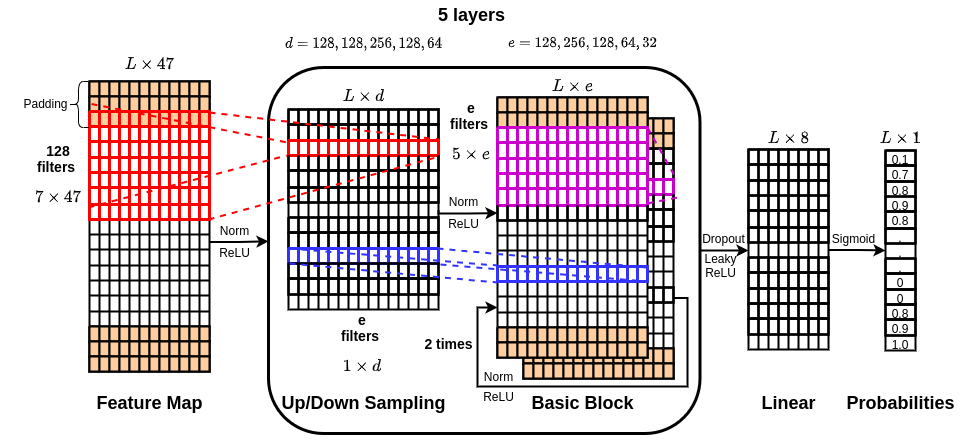
\includegraphics[scale=0.37]{architecture}
    \label{fig:architecture}
\end{figure}

The feature vector is passed through the first level which consists of a 1D convolutional layer with 128 filters, each filter size being 7, a batch normalization layer and the ReLU (Rectified Linear Unit) activation function. The input is padded with zeroes to ensure that the length of the output vector remains the same. The filters of the convolution layer stride across the length of the protein, considering the features of the 3 amino acids before, the 3 amino acids after and the current amino acid (totalling 7). This allows for the extraction of required information of the current amino acid based on the features of nearby amino acids.

The next few levels consist of 2 blocks called BasicBlocks. A BasicBlock consists of a 1D convolutional layer, a batch normalization layer, a ReLU activation function, a second 1D convolutional layer, a second batch normalization layer, and a final ReLU activation. The skip connection is done after the final ReLU activation, where the initial input to the BasicBlock is simply added to the output of the final ReLU activation. Usually, the input and output size of the first BasicBlock do not match and hence there is an up/down-sampling layer that ensures that the input has the same shape as that of the output. The output from the previous level passes through the first BasicBlock which has an up/down-sampling layer and then goes through the second BasicBlock. In the proposed architecture, the number of filters used at each level goes from $128 \to 256 \to 128 \to 64 \to 32$, with the filter size being 5 for every convolution.

The last two levels contain a simple, linear, fully-connected artificial neural network. The last but one level has a LeakyReLU activation function along with a dropout as well. The last level has a Sigmoid function at the end to ensure that the output of the model is between $[0, 1]$. The final output of the model is a vector of size $L$ (length of the protein), denoting the probabilities of a residue being a part of the binding site.

\subsubsection{Loss Function}
\quad For model training, the loss function is given by
$L(\hat{y}, y) = -(\alpha\hat{y}\log(y) + (1-\hat{y})\log(1-y))$, where $\hat{y}$ is the vector of true labels of whether an amino acid belongs to the binding site or not, $y$ is the model output of probabilities of a residue belonging to a binding site, $\alpha$ is the weight that is assigned to the rare class.

The main problem in this classification task is the heavy imbalance in the 2 classes of binding and non-binding residues. As shown in table \ref{tab:dataset_summary}, the percentage of binding residues is only around 6\%. Hence, $\alpha$ is used to penalize the model more heavily if it incorrectly predicts binding residues. $\alpha$ is calculated on the fly for every batch of inputs as $\alpha = \frac{n_{nbr}}{n_{br}}$, where $n_{nbr}$ is the total number of non-binding residues in the batch and $n_{br}$ is the total number of binding residues in the batch.

\subsubsection{Implementation}
\quad The model is implemented using PyTorch Lightning \cite{falcon2019pytorch}, which is a wrapper on the popular open-source deep learning library, PyTorch \cite{NEURIPS2019_9015}. The implementation can be found at \href{https://github.com/crvineeth97/protein-binding-site-prediction}{https://github.com/crvineeth97/protein-binding-site-prediction}.

\newpage
\section{Results}
\quad The sc-PDB dataset was split into ten folds, and ten models with the same architecture were trained. One fold formed the validation set and the remaining folds
formed the training set for each of the models. The validation results are provided in table \ref{tab:results}, along with the confusion matrix in figure \ref{fig:valid_cm}

For testing, the 10 trained models are run on the test set. For consensus, an amino acid belongs to the binding site if 5 or more models predict the same. The test results are also provided in table \ref{tab:results}, along with the confusion matrix in figure \ref{fig:test_cm}

\subsection{Evaluation Metrics}
\subsubsection{Confusion Matrix}
A confusion matrix is a table that allows for the visualization of the performance of a supervised learning algorithm. In the case of binary classification of a residue as a binding residue (BR) or non-binding residue (NBR), the following terminologies can be defined.
\begin{itemize}
    \item True Positive (TP): Number of BRs predicted correctly as BRs.
    \item True Negative (TN): Number of NBRs predicted correctly as NBRs.
    \item False Positive (FP): Number of NBRs predicted incorrectly as BRs.
    \item False Negative (FN): Number of BRs predicted incorrectly as NBRs.
\end{itemize}

\noindent The following metrics can be derived from the confusion matrix

Accuracy: ${ACC} = \frac{TP + TN}{TP + TN + FP + FN}$

Precision: ${PPV} = \frac{TP}{TP + FP}$

Recall: ${TPR} = \frac{TP}{TP + FN}$

F1 score: ${F_1} = \frac{2TP}{2TP + FP + FN}$

Matthews Correlation Coefficient: ${MCC} = \frac{TP \times TN - FP \times FN}{\sqrt{(TP + FP)(TP + FN)(TN + FP)(TN + FN)}}$

\begin{table}
    \centering
    \begin{tabular}{| P{2cm} | P{2cm} | P{2cm} | P{2cm} | P{2cm} | P{2cm} |}
        \hline
        Dataset & ACC(\%) & PPV(\%) & TPR(\%) & F1(\%) & MCC(\%) \\
        \hline
        Fold 1  & 92.58   & 48.64   & 70.65   & 57.62  & 54.83   \\
        Fold 2  & 92.18   & 46.80   & 67.29   & 55.20  & 52.08   \\
        Fold 3  & 92.94   & 44.85   & 69.37   & 54.48  & 52.27   \\
        Fold 4  & 91.28   & 39.62   & 65.73   & 49.44  & 46.72   \\
        Fold 5  & 91.74   & 46.33   & 73.11   & 56.72  & 54.07   \\
        Fold 6  & 92.19   & 47.16   & 69.70   & 56.25  & 53.34   \\
        Fold 7  & 91.90   & 45.45   & 69.55   & 54.98  & 52.13   \\
        Fold 8  & 92.52   & 47.58   & 68.16   & 56.04  & 53.10   \\
        Fold 9  & 92.06   & 41.86   & 69.69   & 52.31  & 50.14   \\
        Fold 10 & 92.08   & 44.54   & 68.88   & 54.10  & 51.41   \\
        Test    & 94.05   & 50.46   & 67.45   & 57.73  & 55.27   \\
        \hline
    \end{tabular}
    \caption{\label{tab:results} Validation results of all 10 trained models and test results}
\end{table}

\begin{figure}
    \caption{\centering Sum of confusion matrices of the 10 models on their corresponding validation set}
    \centering
    \noindent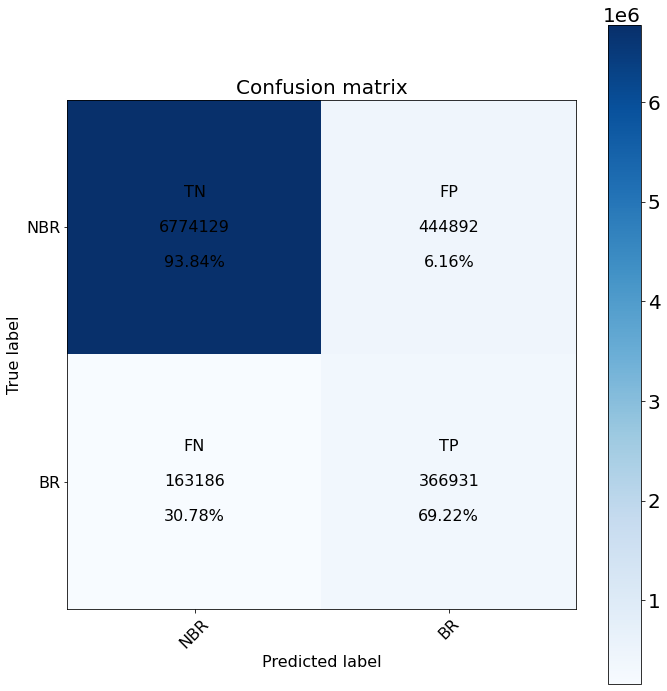
\includegraphics[scale=0.4]{valid_cm.png}
    \label{fig:valid_cm}
\end{figure}
\begin{figure}
    \caption{\centering Confusion matrix on the test set after averaging the predictions of the 10 models}
    \centering
    \noindent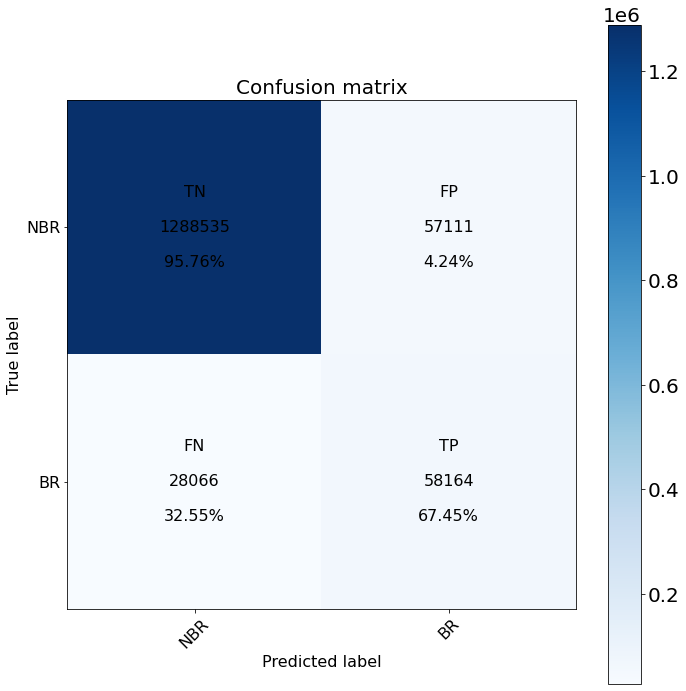
\includegraphics[scale=0.4]{test_cm.png}
    \label{fig:test_cm}
\end{figure}


\subsubsection{DCC}
DCC is the distance between the center of the predicted binding pocket and the center of the true binding pocket. It is commonly used for evaluating 3D-structure based models. The success rate of DCC is defined as the fraction of predictions below a given threshold. Predicted pockets with DCC below 4{\AA} are considered to be correctly located.The model predictions were mapped back to the available 3D structures of proteins for the calculation of DCC.

Figure \ref{fig:valid_dcc} denotes the cross-validation results. The deep learning model is the same across all 10 splits of training and validation datasets. The success rate of the models vary based on the fold that is used for validation. It ranges from 33\% to 49\% success rate when the DCC threshold is less than 4\AA. Figure \ref{fig:test_dcc} denotes the test result. The predictions have a 40\% success rate when the DCC threshold is less than 4\AA.

\vspace{10 mm}
\begin{figure}
    \caption{\centering Success rate plot for various DCC thresholds of the 10 models on their corresponding validation set}
    \centering
    \noindent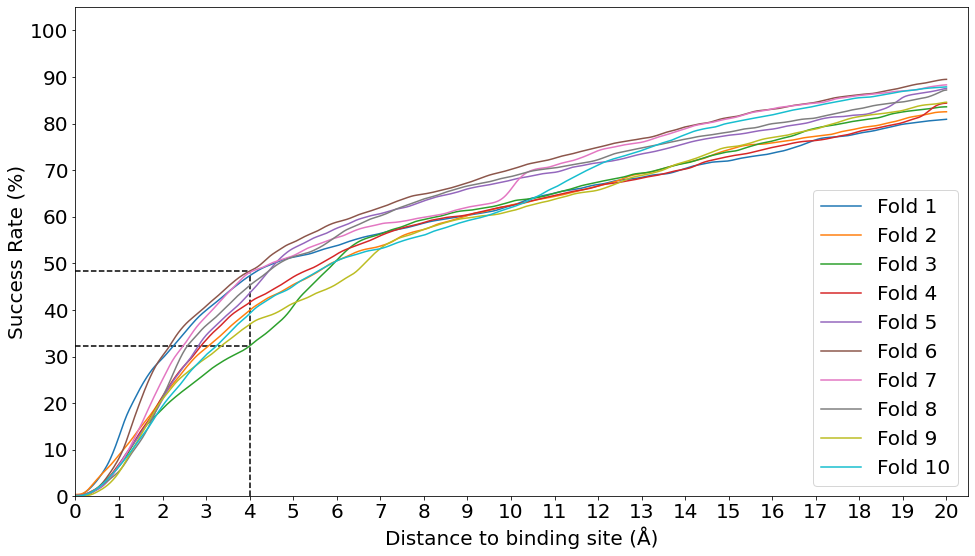
\includegraphics[scale=0.45]{valid_dcc.png}
    \label{fig:valid_dcc}
\end{figure}

\begin{figure}
    \caption{\centering Success rate plot for various DCC thresholds on the test set after averaging the predictions of the 10 models}
    \centering
    \noindent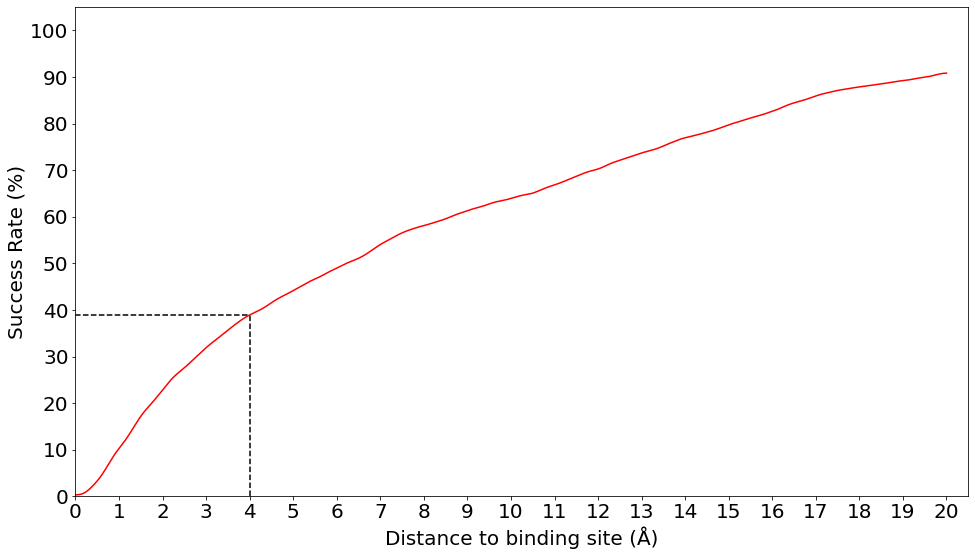
\includegraphics[scale=0.45]{test_dcc.png}
    \label{fig:test_dcc}
\end{figure}

% \subsection{Experiments}
% \quad Should all the things that I tried be included? For eg.

% TAPE Embeddings (Both embeddings) and as a downstream task

% Complementary GAN to try and solve the imbalance

% Using SPOT-1D features

% BiLSTMs, UNet, Transformers

% Window of features using predicted contact maps

% Training on chains separately


\section{Discussion}
\quad The Matthew's Correlation varies from $[-1, +1]$, with $+1$ representing a perfect prediction, 0 representing no better than a random prediction and -1 representing total disagreement between the prediction and the observation. The MCC on the test set seems to be ranging from -0.11 to +1, which may seem surprising at first, but actually shows the effectiveness of the model.

\subsection{Case Studies}
\quad The aggregated predictions of the models on the test set were mapped back to the three-dimensional structure of the protein-ligand complex to see how good the predictions are. In the following examples, the colour red indicates an incorrect prediction of the amino acid as a binding residue, blue indicates an amino acid that is actually a binding residue but was not predicted as binding by the model and green indicates an amino acid that was correctly predicted as binding.

\subsubsection{5YMX}
\quad In figure \ref{fig:5ymx}, it looks like the model is predicting everything incorrectly, but, it is actually predicting another binding site of the protein! The sc-PDB dataset was generated through a series of filters and the residues surrounding the most buried ligand was selected to be the most ligandable binding site. This, unfortunately, is a flaw of the dataset and the method used for predictions. There isn't a good way to cover cases like these where the model needs to be penalized less when it predicts a binding site that isn't the most ligandable binding site. Hence, the evaluation metrics used will generally give a very poor score for such cases.
\begin{figure}
    \caption{\centering 5YMX}
    \centering
    \noindent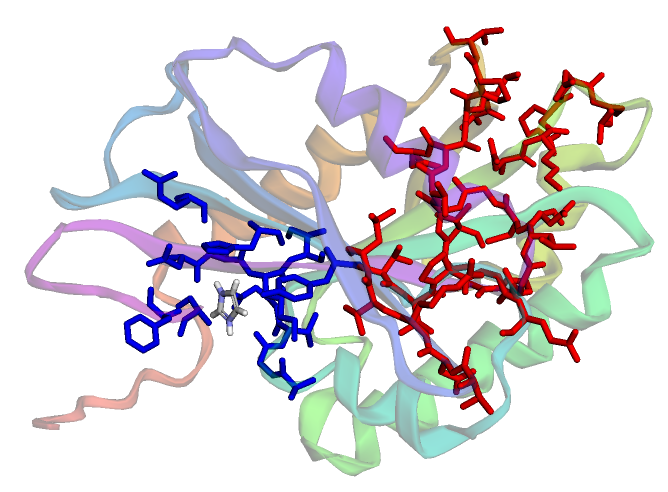
\includegraphics[scale=0.45]{5ymx.png}
    \label{fig:5ymx}
\end{figure}

\subsubsection{6HU9}
\quad Figure \ref{fig:6hu9} shows an example where the model predicts individual binding sites of 2 proteins with the same sequence, but, it finds it difficult to predict the binding site made due to the interaction between the 2 proteins. 
\begin{figure}
    \caption{\centering 6HU9}
    \centering
    \noindent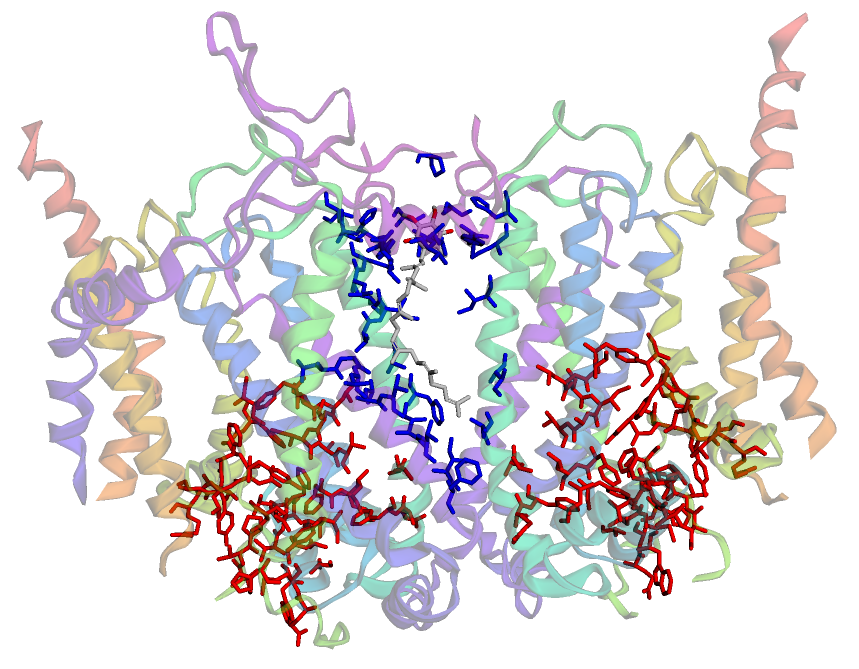
\includegraphics[scale=0.4]{6hu9.png}
    \label{fig:6hu9}
\end{figure}

\subsection{Areas for Improvement}
\quad 

%%%%%%%%%%%%%%%%%%%%%%%%%%%%%%%%%%%%%%%%%%%%%%%%%%%%%%%%%%%%%%%%%%%%%
%% The "Acknowledgement" section can be given in all manuscript
%% classes.  This should be given within the "acknowledgement"
%% environment, which will make the correct section or running title.
%%%%%%%%%%%%%%%%%%%%%%%%%%%%%%%%%%%%%%%%%%%%%%%%%%%%%%%%%%%%%%%%%%%%%
\begin{acknowledgement}
    The author thanks Yashaswi Pathak for being a fruitful part of the project discussions.

\end{acknowledgement}

%%%%%%%%%%%%%%%%%%%%%%%%%%%%%%%%%%%%%%%%%%%%%%%%%%%%%%%%%%%%%%%%%%%%%
%% The same is true for Supporting information, which should use the
%% suppinfo environment.
%%%%%%%%%%%%%%%%%%%%%%%%%%%%%%%%%%%%%%%%%%%%%%%%%%%%%%%%%%%%%%%%%%%%%
\begin{suppinfo}

    This will usually read something like: ``Experimental procedures and
    characterization data for all new compounds. The class will
    automatically add a sentence pointing to the information on-line:

\end{suppinfo}

%%%%%%%%%%%%%%%%%%%%%%%%%%%%%%%%%%%%%%%%%%%%%%%%%%%%%%%%%%%%%%%%%%%%%
%% The appropriate \bibliography command should be placed here.
%% Notice that the class file automatically sets \bibliographystyle
%% and also names the section correctly.
%%%%%%%%%%%%%%%%%%%%%%%%%%%%%%%%%%%%%%%%%%%%%%%%%%%%%%%%%%%%%%%%%%%%%
\bibliography{achemso-demo}

\end{document}